\documentclass[a4paper]{article}

\usepackage{pgfplots}
%\usepackage{tikz}

\usepgfplotslibrary{fillbetween}
\usepgfplotslibrary{patchplots}



\begin{document}



% We use the polynomial f(x) -1/100 x^2 +2x .

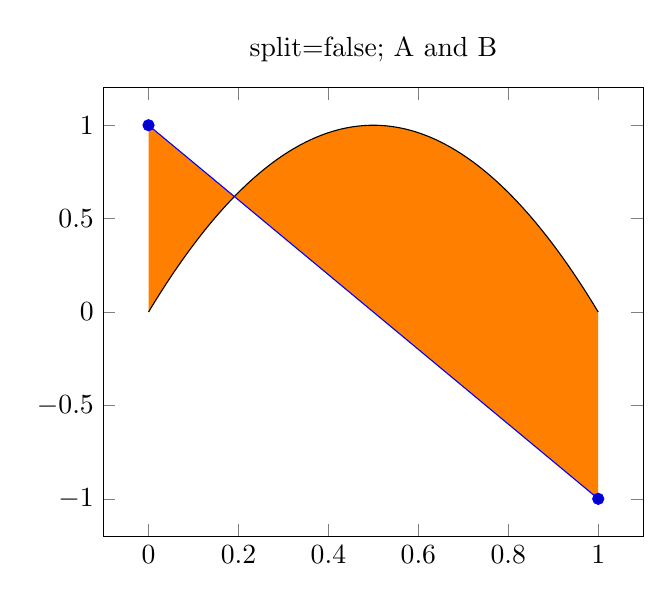
\begin{tikzpicture}
	\begin{axis}[title={split=false; A and B}]
	\draw[name path=A] (axis cs:0,0) .. controls (axis cs:0.333,1.3333) and (axis cs:0.66666,1.33333) .. (axis cs:1,0);
	
	%
	%\addplot+[name path=A,patch, point meta=none,patch type=quadratic spline]
	%	coordinates {(0,0) (1,0) (0.5,1)};
	
	\addplot+[name path=B] coordinates {(0,1) (1,-1)};

	\addplot[orange] fill between[of=A and B];
	\end{axis}
\end{tikzpicture}
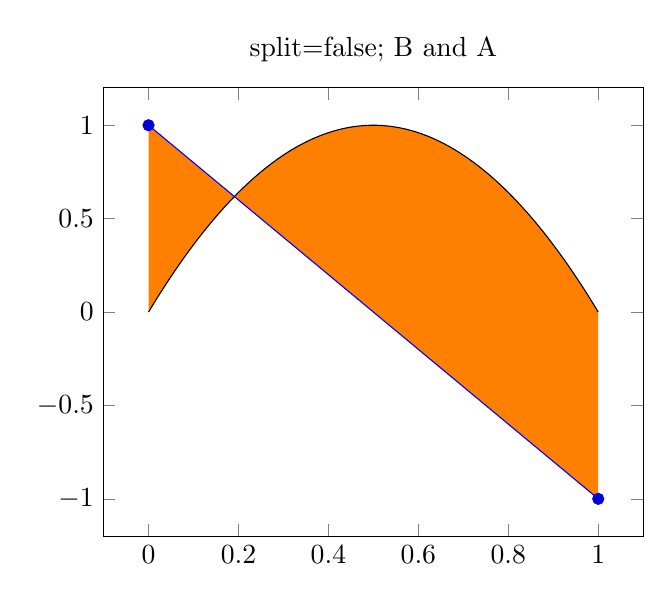
\begin{tikzpicture}
	\begin{axis}[title={split=false; B and A}]
	\draw[name path=A] (axis cs:0,0) .. controls (axis cs:0.333,1.3333) and (axis cs:0.66666,1.33333) .. (axis cs:1,0);
	
	%
	%\addplot+[name path=A,patch, point meta=none,patch type=quadratic spline]
	%	coordinates {(0,0) (1,0) (0.5,1)};
	
	\addplot+[name path=B] coordinates {(0,1) (1,-1)};

	\addplot[orange] fill between[of=B and A];
	\end{axis}
\end{tikzpicture}

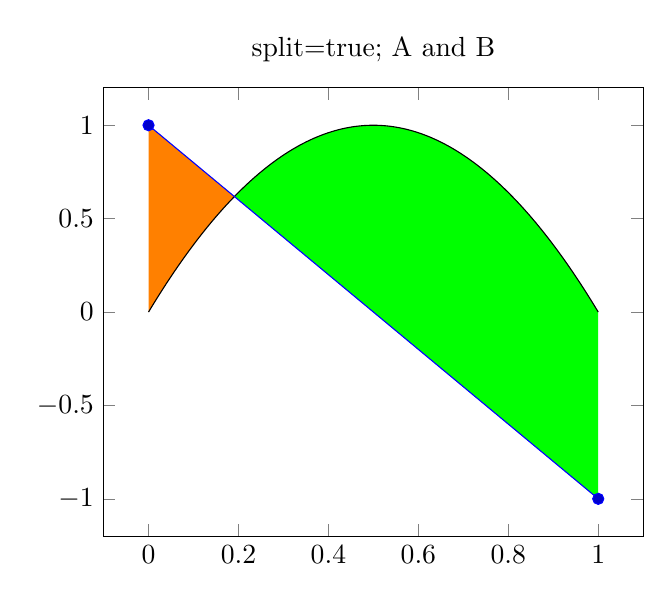
\begin{tikzpicture}
	%\tracingmacros=2 \tracingcommands=2
	\begin{axis}[title={split=true; A and B}]
	\draw[name path=A] (axis cs:0,0) .. controls (axis cs:0.333,1.3333) and (axis cs:0.66666,1.33333) .. (axis cs:1,0);
	
	\addplot+[name path=B] coordinates {(0,1) (1,-1)};

	\addplot[orange] fill between[%
		of=A and B,split,
		every odd segment/.style={green},
	];
	\end{axis}
\end{tikzpicture}
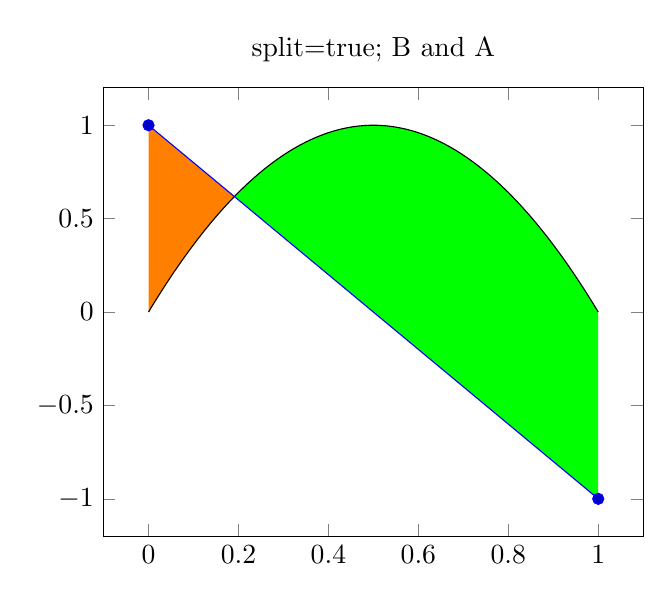
\begin{tikzpicture}
	%\tracingmacros=2 \tracingcommands=2
	\begin{axis}[title={split=true; B and A}]
	\draw[name path=A] (axis cs:0,0) .. controls (axis cs:0.333,1.3333) and (axis cs:0.66666,1.33333) .. (axis cs:1,0);
	
	\addplot+[name path=B] coordinates {(0,1) (1,-1)};

	\addplot[orange] fill between[%
		of=B and A,split,
		every odd segment/.style={green},
	];
	\end{axis}
\end{tikzpicture}

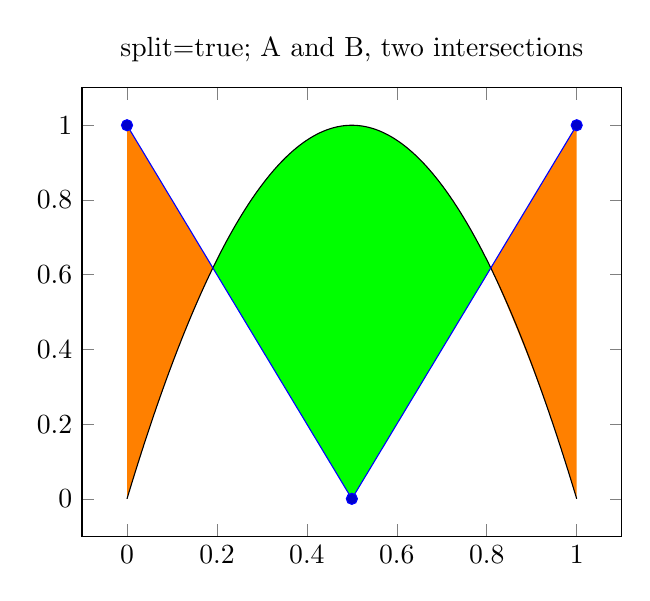
\begin{tikzpicture}
	%\tracingmacros=2 \tracingcommands=2
	\begin{axis}[title={split=true; A and B, two intersections}]
	\draw[name path=A] (axis cs:0,0) .. controls (axis cs:0.333,1.3333) and (axis cs:0.66666,1.33333) .. (axis cs:1,0);
	
	\addplot+[name path=B] coordinates {(0,1) (0.5,0) (1,1)};

	\addplot[orange] fill between[%
		of=A and B,split,
		every odd segment/.style={green},
	];
	\end{axis}
\end{tikzpicture}

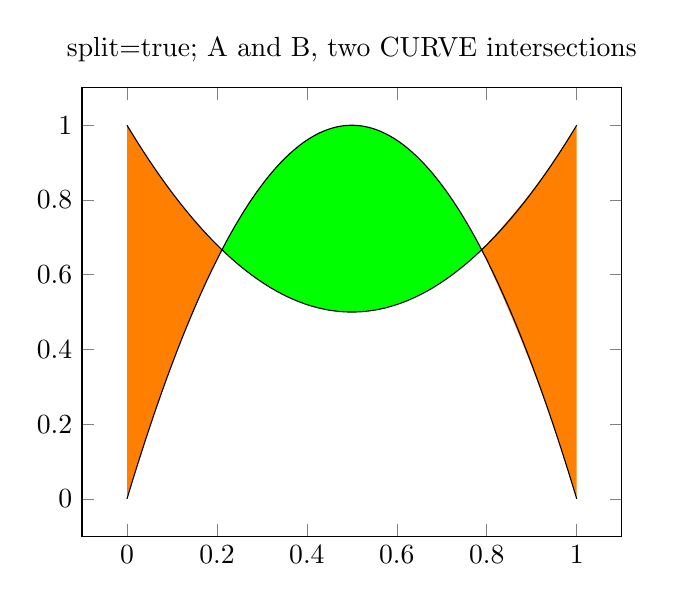
\begin{tikzpicture}
	%\tracingmacros=2 \tracingcommands=2
	\begin{axis}[title={split=true; A and B, two CURVE intersections},
		xmin=0,xmax=1,ymin=0,ymax=1,enlargelimits]
	\draw[name path=A] (axis cs:0,0) .. controls (axis cs:0.333,1.3333) and (axis cs:0.66666,1.33333) .. (axis cs:1,0);
	
	\draw[name path=B] (axis cs:0,1) .. controls (axis cs:0.333,0.3333) and (axis cs:0.66666,0.33333) .. (axis cs:1,1);

	\addplot[orange] fill between[%
		of=A and B,split,
		every odd segment/.style={green},
	];
	\end{axis}
\end{tikzpicture}
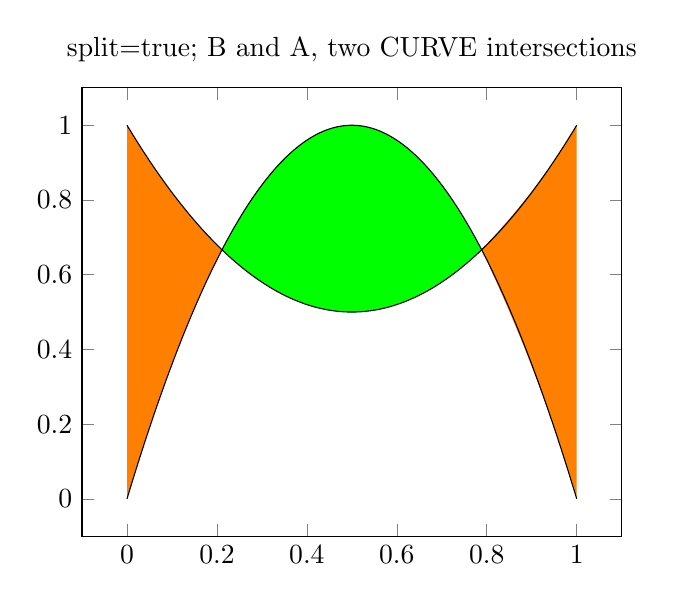
\begin{tikzpicture}
	%\tracingmacros=2 \tracingcommands=2
	\begin{axis}[title={split=true; B and A, two CURVE intersections},
		xmin=0,xmax=1,ymin=0,ymax=1,enlargelimits]
	\draw[name path=A] (axis cs:0,0) .. controls (axis cs:0.333,1.3333) and (axis cs:0.66666,1.33333) .. (axis cs:1,0);
	
	\draw[name path=B] (axis cs:0,1) .. controls (axis cs:0.333,0.3333) and (axis cs:0.66666,0.33333) .. (axis cs:1,1);

	\addplot[orange] fill between[%
		of=B and A,split,
		every odd segment/.style={green},
	];
	\end{axis}
\end{tikzpicture}



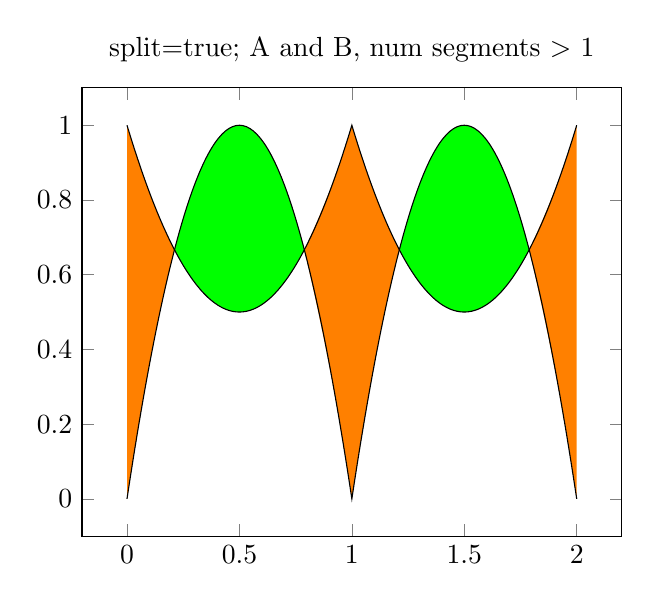
\begin{tikzpicture}
	%\tracingmacros=2 \tracingcommands=2
	\begin{axis}[title={split=true; A and B, num segments $>$ 1},
		xmin=0,xmax=2,ymin=0,ymax=1,enlargelimits]
	\draw[name path=A] 
		(axis cs:0,0) 
		.. controls (axis cs:0.333,1.3333) and (axis cs:0.66666,1.33333) .. (axis cs:1,0)
		.. controls (axis cs:1.333,1.3333) and (axis cs:1.66666,1.33333) .. (axis cs:2,0)
	;
	
	\draw[name path=B] (axis cs:0,1) 
		.. controls (axis cs:0.333,0.3333) and (axis cs:0.66666,0.33333) .. (axis cs:1,1)
		.. controls (axis cs:1.333,0.3333) and (axis cs:1.66666,0.33333) .. (axis cs:2,1)
	;

	\addplot[orange] fill between[%
		of=A and B,split,
		every odd segment/.style={green},
	];
	\end{axis}
\end{tikzpicture}


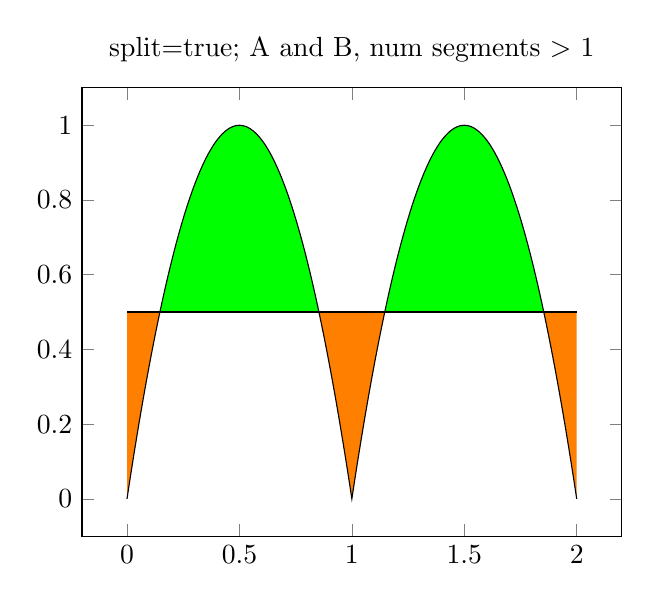
\begin{tikzpicture}
	%\tracingmacros=2 \tracingcommands=2
	\begin{axis}[title={split=true; A and B, num segments $>$ 1},
		xmin=0,xmax=2,ymin=0,ymax=1,enlargelimits]
	\draw[name path=A] 
		(axis cs:0,0) 
		.. controls (axis cs:0.333,1.3333) and (axis cs:0.66666,1.33333) .. (axis cs:1,0)
		.. controls (axis cs:1.333,1.3333) and (axis cs:1.66666,1.33333) .. (axis cs:2,0)
	;
	
	\draw[name path=B] (axis cs:0,0.5) -- (axis cs:1,0.5) -- (axis cs:2,0.5)
	;

	\addplot[orange] fill between[%
		of=A and B,split,
		every odd segment/.style={green},
	];
	\end{axis}
\end{tikzpicture}
\end{document}


